\section{Analysis of the effects of pose normalization}

The original model of the 3D pose estimation system by \citet{drover18}, which is described in Section \ref{sec:network}, requires the input pose to be normalized in the following way:
\begin{enumerate}[label=(\Alph*)]
	\item The 2D input pose's root joint is centered at the origin.
	\item A designated norm limb has length 0.1.
\end{enumerate}

In reality both assumptions are rarely satisfied from the start.
Thus \citet{drover18} normalize the input 2D poses by shifting and scaling before feeding them to the generator.
In this chapter we will see both theoretically and experimentally that this approach inevitably leads to additional errors being introduced to the system.

\Todo[inline]{Figure of camera projection}

In the following we will assume that the camera used for projection is located at the origin of the coordinate system and looks into positive z direction.
All poses are assumed to have z coordinates greater than camera's focal length $f$ in order to be projected in front of the camera.
The generator $G$ will be regarded as a black box that takes a normalized 2D pose as input and outputs the depths (the z coordinates) of the input points which then can be reprojected into three dimensional space like in Equation \eqref{eq:perspective-re-projection}.

\Todo[inline]{
For simplicity, the problem will only be regarded in two dimensions.
For three dimensions the y coordinates are to be inserted at the appropriate places.
}

\subsection{Shifting along one image plane axis}
\label{sec:x-shift-error}
First we will analyze assumption (A) by examining a 3D pose $P$ which is centered at the origin of the x-y-plane.
$P$ is then shifted by the vector $(dx, dy, 0)$ along the x-y-plane and projected into two dimensions.
After the 2D pose has been aligned with the image plane's origin, it is re-projected into three dimensions.
The resulting 3D pose $\widetilde{P}$ will then be compared to the original 3D pose $P$ in order to gain insights in the additional error made through normalization.

Let $P = [(X_1, Y_1, Z_1), \dotsc, (X_n, Y_n, Z_n)]$ be a 3D pose.
For simplicity we will assume that $dy = 0$, that is, the pose $P$ is only shifted along the x axis.

\subsubsection{Theoretical analysis}
\label{sec:x-shift-error-theoretical}
Let $P_i = (X_i, Y_i, Z_i) \in P$.
Then the coordinates of the projected point on the image plane are given by
\begin{equation}
	x_i = f \frac{X_i}{Z_i} \ ,\enspace y_i = f \frac{Y_i}{Z_i} \ .
\end{equation}
Now assume that $P_i$ is shifted by $dx$ along the x axis.
This results in a projected x coordinate of
\begin{equation}
	x_i^\mathrm{S} = f \frac{X_i + dx}{Z_i} = f \frac{X_i}{Z_i} + f \frac{dx}{Z_i} = x_i + f \frac{dx}{Z_i}\ .
\end{equation}
The projected pose is then normalized by shifting all projected points such that the root node is located in the origin of the image plane. 
Let the shifted root node have coordinates $(dx, 0, Z)$.
Since $dy = 0$, each point is only shifted by $- f \frac{dx}{Z}$ along the x axis.
That means the x coordinate of the normalized point $\widetilde{x}_i$ is given by
\begin{equation}
	\widetilde{x}_i
	= x_i^\mathrm{S} - f \frac{dx}{Z}
	= x_i + f \frac{dx}{Z_i} - f \frac{dx}{Z}
	= x_i + f dx (\frac{1}{Z_i} - \frac{1}{Z})\ .
\end{equation}
After $G$ estimates the depth $\widetilde{Z}_i$, it is reprojected into three dimensions. The resulting coordinates are 
\begin{align}
	\label{eq:re-projected-X}
	\widetilde{X}_i &= \frac{\widetilde{x}_i}{f} \cdot \widetilde{Z}_i
	= X_i \frac{\widetilde{Z}_i}{Z_i} + dx (\frac{1}{Z_i} - \frac{1}{Z}) \widetilde{Z}_i
	= \widetilde{Z_i} \left( \frac{X_i}{Z_i} + dx \left( \frac{1}{Z_i} - \frac{1}{Z} \right) \right) \ , \\
	\label{eq:re-projected-Y}
	\widetilde{Y}_i &= \frac{y_i}{f} \cdot \widetilde{Z}_i = \frac{Y_i}{Z_i} \cdot \widetilde{Z}_i \ .
\end{align}
The Euclidean distance (the Joint Position Error (JPE)) of the reprojected point to the original point is given by
\begin{equation}
\label{eq:delta-d}
	\Delta d_i = \norm{ 
	\begin{pmatrix}
		\widetilde{X}_i - X_i \\
		\widetilde{Y}_i - Y_i \\
		\widetilde{Z}_i - Z_i
	\end{pmatrix}
	}_2
\end{equation}
With perfect estimation of $\widetilde{Z_i} = Z_i$, we have $\widetilde{Y}_i = Y_i$ and Equation \eqref{eq:delta-d} together with \eqref{eq:re-projected-X} describes a linear relationship between the offset $dx$ and the Joint Position Error $\Delta d_i$.
But since the generator's estimation of $\widetilde{Z_i}$ can vary for different offsets $dx$, the JPE can actually become smaller for other $\widetilde{Z_i} \neq Z_i$. 
In order to obtain a correct lower bound for the Joint Position Error, we have to calculate the $\widetilde{Z_i}$ for which $\Delta d_i$ is minimal.
So the function to be minimized is
\begin{align}
	\label{eq:minimum-distance}
	f(\widetilde{Z}_i) &= \left ( \widetilde{Z}_i \cdot \left( \frac{X_i}{Z_i} + dx \left( \frac{1}{Z_i} - \frac{1}{Z} \right) \right ) - X_i \right)^2 + \left ( \widetilde{Z_i} \cdot \frac{Y_i}{Z_i} - Y_i \right )^2 + \left ( \widetilde{Z}_i - Z_i \right ) ^2 \\
	&= \left ( \widetilde{Z}_i \cdot a - X_i \right)^2 + \left ( \widetilde{Z_i} \cdot b - Y_i \right )^2 + \left ( \widetilde{Z}_i - Z_i \right )^2 \ ,
\end{align}
where $a \coloneqq \left( \frac{X_i}{Z_i} + dx \left( \frac{1}{Z_i} - \frac{1}{Z} \right) \right )$ and $b \coloneqq \frac{Y_i}{Z_i}$ have been substituted for better readability.
In order to obtain the optimal value for $\widetilde{Z}_i$, $f$ is differentiated by $\widetilde{Z}_i$:
\begin{equation}
	\label{eq:derivative-minimum-distance}
	f'(\widetilde{Z}_i) = 2 \cdot \left ( \widetilde{Z}_i \left (a^2 + b^2 \right ) - a X_i - b Y_i + \widetilde{Z}_i - Z_i \right )
\end{equation}
Setting this equal to zero gives
\begin{align}
	0 &= f'(\widetilde{Z}_i^\ast) \\
	\Leftrightarrow \widetilde{Z}_i^\ast & = \frac{a X_i + b Y_i + Z_i}{1 + a^2 + b^2} \ .
	\label{eq:z_i-min}
\end{align}
As $f$ converges towards infinity for $\widetilde{Z_i} \rightarrow \pm \infty$, it is easy to see that $\widetilde{Z}_i^\ast$ is $f$'s only extremum; a minimum.
With $\widetilde{Z}_i^\ast$ the optimal $\widetilde{X}_i^\ast$ and $\widetilde{Y}_i^\ast$ from Equation \eqref{eq:re-projected-X} and \eqref{eq:re-projected-Y} can now be calculated:
\begin{align}
	\label{eq:x_i-min}
	\widetilde{X}_i^\ast &= \widetilde{Z}_i^\ast \cdot a
	= \frac{a^2 X_i + a b Y_i +  a Z_i}{1 + a^2 + b^2} \ ,\\
	\label{eq:y_i-min}
	\widetilde{Y}_i^\ast &= \widetilde{Z}_i^\ast \cdot b
	= \frac{b^2 Y_i + a b X_i + b Z_i}{1 + a^2 + b^2} \ . 
\end{align}

Putting \eqref{eq:z_i-min}, \eqref{eq:x_i-min} and \eqref{eq:y_i-min} into \eqref{eq:delta-d} yields a total minimal error of 
\begin{align}
	\Delta d_i &= 
	\sqrt{\left (\widetilde{X}_i^\ast - X_i \right )^2 + \left (\widetilde{Y}_i^\ast - Y_i \right )^2 + \left (\widetilde{Z}_i^\ast - Z_i \right )^2}\\
	& = \sqrt{\frac{\left (a Y_i - b X_i \right )^2 + \left (a Z_i - X_i \right )^2 + \left (b Z_i - Y_i \right )^2}{1 + a^2 + b^2}} \\
	\label{eq:bzy-zero}
	&= \sqrt{\frac{\left (dx \cdot Y_i \cdot \left (\frac{1}{Z_i} - \frac{1}{Z} \right) \right)^2 + \left (a Z_i - X_i \right )^2}{1 + a^2 + b^2}}\\
	& = \sqrt{\frac{\left (dx \cdot Y_i \cdot \left (\frac{1}{Z_i} - \frac{1}{Z} \right ) \right)^2 + \left (dx \cdot Z_i \cdot \left (\frac{1}{Z_i} - \frac{1}{Z} \right ) \right)^2}{1 + a^2 + b^2}} \\
	& = \sqrt{\frac{dx^2 \cdot \left (\frac{1}{Z_i} - \frac{1}{Z} \right )^2 \cdot \left (Y_i^2 + Z_i^2 \right ) }{1 + a^2 + b^2}}\\
	\label{eq:minimum-delta-d}
	& = \abs{dx \left (\frac{1}{Z_i} - \frac{1}{Z} \right )} \sqrt{\frac{(Y_i^2 + Z_i^2)}{1 + a^2 + b^2}} \ .
\end{align}
In Equation \eqref{eq:bzy-zero} $b Z_i - Y_i = 0$ has been used.
With this $\Delta d_i$ the MPJPE for the whole pose can then be calculated as the mean of all $\Delta d_i$s:
\begin{equation}
	\label{eq:minimum-mpjpe-on-shift}
	\Delta d = \frac{1}{n} \sum_{i = 1}^{n} \Delta d_i 
\end{equation}
In contrast to the linear relationship for $\widetilde{Z_i} = Z_i$, for optimal $\widetilde{Z_i}$, the minimal MPJPE converges to a constant for large $dx$.

This result shows that even with the generator estimating the depth of each point perfectly, the estimated 3D pose will never exactly match the original 3D pose up to shifting and scaling.
Especially the re-projection of the 2D poses into three dimensional space without first shifting the 2D poses back as they were before normalization adds an essential part to the MPJPE.
In fact, the effects of 2D pose normalization by shifting only vanish if $dx = 0$ or $Z_i = Z$ for all $(X_i, Y_i, Z_i) \in P$. In the latter case all joints of the pose are located in a plane parallel to the image plane.

The theoretical results above also show another downside of normalization by shifting.
In case the generator is trained with 2D poses which have multiple different offsets $dx$ and $dy$, ambiguities are introduced to the system:
As the generator can't know whether the pose it receives was originally located in the origin of the image plane or not, it can't correctly learn which depth offset belongs to which pose.
\unsure{Should possible solutions already presented here?}
One easy solution for this second problem is to train only with poses that all have the same offsets in x and y direction.
As this is rarely the case in reality, that would make the system only viable for very specific tasks in practice.

\unsure{Mention the intuition behind the phenomenon: Shift means we see the pose more from the side.}

\subsubsection{Experimental results}

In this section the observable MPJPEs of shifted poses will be compared to the theoretical results above. 
Figure \ref{fig:x-shift-error} depicts a plot of the MPJPEs (measured using Protocol 2; Section \ref{sec:protocol2}) for 2D poses sampled from subjects 9 and 11 with different offsets in x direction along with a plot of the minimal MPJPE calculated in Equation \eqref{eq:minimum-mpjpe-on-shift}.
As it turns out, both curves have the same approximate shape, but the sampled poses' MPJPE is significantly smaller than the theoretical MPJPE.
The discrepancy between the curves is increasing for larger offsets $\abs{dx}$.
At first glance, this seemingly contradicts the fact that the above $\Delta d$ represents a lower bound for the error.

But one important detail has not been taken into account yet:
During the evaluation with Protocol 2, shifting and scaling might be applied to the estimated poses. 
For the root joint $r$ we have $Z_i = Z$ in \eqref{eq:minimum-delta-d}, so $\Delta d_r = 0$. That means $(\widetilde{X}_i, \widetilde{Y_i}, \widetilde{Z}_i) = (X_i, Y_i, Z_i)$, that is, the root nodes of both poses are already aligned.
It is not as easy to make a statement about scale of the pose $\widetilde{P}$ from a theoretical point of view only though.
Experimental results show that the average limb length of $\widetilde{P}$ is increasing monotonously with increasing offset $\abs{dx}$.
That means with Protocol 2 each pose $\widetilde{P}$ is re-scaled by a factor $\alpha_{\widetilde{P}}$ in all dimensions before the MPJPE is calculated, so
\begin{equation}
	\Delta d_i = \norm{ 
	\begin{pmatrix}
		\alpha_{\widetilde{P}} \cdot \widetilde{X}_i - X_i \\
		\alpha_{\widetilde{P}} \cdot \widetilde{Y}_i - Y_i \\
		\alpha_{\widetilde{P}} \cdot \widetilde{Z}_i - Z_i
	\end{pmatrix}
	}_2 \ .
\end{equation}

The 

\begin{figure}[ht]	
	\centering
	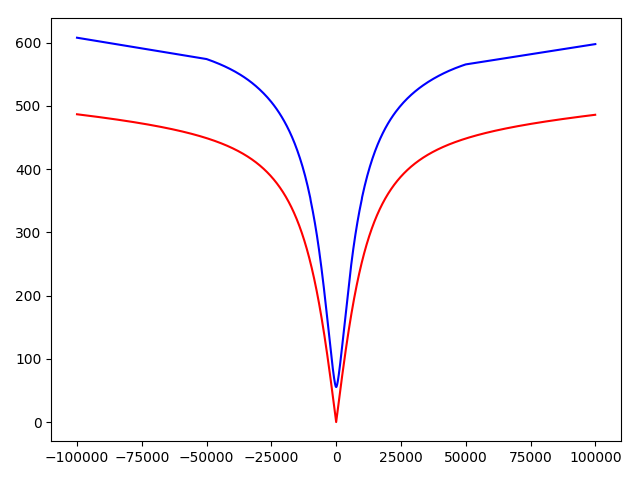
\includegraphics[scale=0.5]{figures/x_shift_error.png}
	\caption{Plot of theoretical (red) and observed (blue) MPJPEs for different values of $dx$. 
		The theoretical errors are obtained by calculating the mean of MPJPES $\alpha \Delta d$ for the evaluation data.}
	\Todo[inline]{Add axes titles, use proper image.
	use pgfplots to plot data}
	\label{fig:x-shift-error}
\end{figure}

It is also noticeable that the performance of the network is not worse than the theoretical results by a constant offset.
For small deviations along the x axis the network seems to be able to compensate the error introduced by shifting.
As $dx$ increases, so does the offset between the observed and the theoretical results until it seems to converge to a constant.
This motivates adjusting not only how the inferred points are reprojected into three dimensions but also network itself.
This will be discussed further in section \ref{sec:network-adjusting}.

As shown in Section \ref{sec:data-results} the MPJPE for the original 2D poses is about \Todo{Check this number} 30mm higher than the one for the synthetically generated data.
The simplest explanation for this is that the original 2D poses do not fulfill the constraints for the system.
The camera is not centered on the root joint and also the camera distance is most certainly not exactly ten times the length of the norm limb.

Numbers: ...
	
\subsection{Shifting along the z axis}
\label{sec:z-shift-error}

In this section, assumption (B) will be analyzed.
It states that a 2D pose's designated norm limb should have length $0.1$ when the pose is fed to the generator.
In case the assumption is not fulfilled from the start, there can be two reasons for this: 
An incorrect focal length $f$ of the camera, or an either to large or to small distance $Z$ between the camera and the 3D pose's root node.

In case $Z$ is fixed for all poses and only the focal length of the camera is incorrect, the pose can be normalized without any problems.
As the focal length is only a scale factor the projected points are multiplied with, dividing by it results in the same 2D pose as if $f$ has been correct in the first place.

But when the focal length $f$ of the camera is fixed and the incorrect length of the norm limb is caused by the distance between the camera and the root node, normalization by scaling will introduce an additional error.
The intuitional explanation behind this is that the projection rays' relative angles change when the 3D pose is projected with greater or smaller distance.
The resulting MPJPE will be analyzed in the following section.

\subsubsection{Theoretical analysis}
Again consider a point $P_i=(X_i, Y_i, Z_i) \in P$ and a camera with focal length $f$. Assume that $P_i$ is shifted by $dz$ along the z axis.
The x coordinate of the projected point on the image plane is
\begin{equation}
	x_i = f \frac{X_i}{Z_i + dz}
\end{equation}
The projected points are now scaled such that they have the same (arbitrary) scale, that is, a norm limb length of 0.1.
Let $\alpha$ be the scale factor of the original projected points and $\beta$ be the one of the shifted projected points. 
The x coordinate of the scaled projected point is given by
\begin{equation}
		\widetilde{x}_i = x_i \cdot \frac{\alpha}{\beta} 
		= f \frac{X_i}{Z_i + dz}\cdot \frac{\alpha}{\beta} 
\end{equation}
After the generator estimates the depth $\widetilde{Z}_i$, the point is re-projected into three dimensional space.
The re-projected point is given by
\begin{equation}
	\widetilde{X}_i = \frac{\widetilde{x}_i}{f} \cdot \widetilde{Z}_i
	= \frac{X_i}{Z_i + dz}\cdot \frac{\alpha}{\beta}  \cdot \widetilde{Z}_i
\end{equation}
Like in Section \ref{sec:x-shift-error-theoretical}, the Euclidean distance to the original point should be minimized with respect to $\widetilde{Z_i}$.
We consider the function
\begin{equation}
	f(\widetilde{Z}_i) = \left ( \widetilde{Z}_i \cdot \frac{X_i}{Z_i + dz}\cdot \frac{\alpha}{\beta} - X_i \right)^2 + ( \widetilde{Z}_i - Z_i )^2 \ .
\end{equation}
If we define $a \coloneqq \frac{X_i}{Z_i + dz}\cdot \frac{\alpha}{\beta}$, we can obtain the same derivative as in Equation \eqref{eq:derivative-minimum-distance}.
So with the same optimal 
\begin{equation}
	\widetilde{Z_i} = \frac{a X_i + Z_i}{1 + a^2} \ ,
\end{equation}
we can obtain a total minimal JPE of 
\begin{equation}
	\label{eq:z-shift-error}
	\Delta d_i = \sqrt{\frac{(a Z_i - X_i)^2}{1 + a^2}} 
	= \abs{\frac{X_i dz}{Z_i + dz}} \sqrt{\frac{1}{1 + a^2}} \ .
\end{equation}
Again, the MPJPE $\Delta d$ of the whole pose $P$ can be calculated as the mean of all $\Delta d_i$s (Equation \eqref{eq:delta-d}).

In contrast to the results of the previous sections, this theoretical result is not as directly applicable to the system.
Before the evaluation with Protocol 2, the root nodes of the estimated and ground truth poses are aligned.
If the generator estimates the depths $\widetilde{Z}_i = Z_i + dz$ for all $i$, the estimated pose $\widetilde{P}$ equals $P$ up to a shift.


In general, there exists no factor $\gamma$ such that $x_i = \widetilde{x_i}$ for all $i$ (to be precise, such factor only exists if for all $i$ $Z_i = \widetilde{Z_i}$).
That means the shifted projected pose and the original projected pose usually do not match.
Thus, if the generator receives poses with different total depths, it can not know with which camera distance the pose has been captured.


\subsubsection{Experimental results}
\label{sec:error-on-shift-experimental}

This phenomenon is also affecting our ground truth data. The poses are all projected with a camera distance $ \text{length-of-norm-limb} \cdot 10$. 
That means the length of the projected norm limb is not exactly $0.1$ but a bit smaller or bigger. 
Like discussed above those projected poses are then normalized. 
The system estimates the depths of the normalized pose and re-projects it assuming a perfect perspective projection. 
It therefore does not consider the effect of small deviations in z direction.
A way to fix this would be to calculate the perfect camera distance for each pose individually before projecting them onto the image plane.
This is not very realistic though since one might be able to determine the camera's distance to a human approximately, but definitely not exactly. This phenomenon therefore is kind of inevitable.

It can be hoped that the generator can compensate for small deviations in $Z$ by itself.
